\section{Aplicação Desktop}

A versão desktop da aplicação contém 5 páginas: inicial, nova música, nova interpretação, tocar música e sobre nós.

\subsection{Página inicial}
Nesta página faz-se uma breve apresentação da aplicação, disponibilizando ligações de interesse para as restantes páginas (ver \autoref{deskindex}).

\begin{figure}[htp]
\centering
\frame{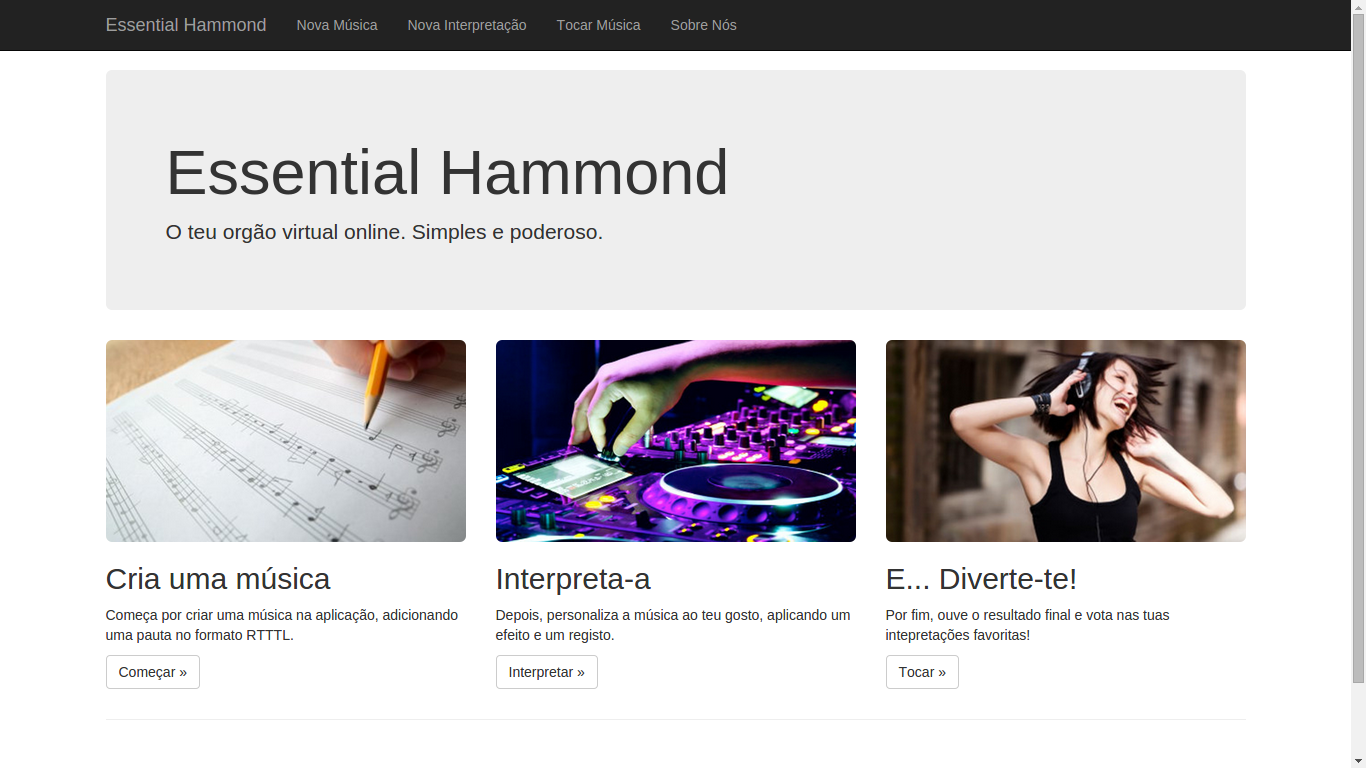
\includegraphics[width=\textwidth]{images/deskindex.png}}
\caption{Página inicial da versão desktop da aplicação.}
\label{deskindex}
\end{figure}

\subsection{Nova música}
Aqui, o utilizador pode adicionar as suas pautas no formato \ac{rtttl} (ver \autoref{desknova}). Para tal, introduz-se a pauta na caixa de texto disponibilizada e carrega-se em enviar música, sendo mostrada uma mensagem de sucesso à direita do botão quando o servidor termina o processamento. É utilizado o serviço /createSong (para enviar a música para o servidor).

\begin{figure}[htp]
\centering
\frame{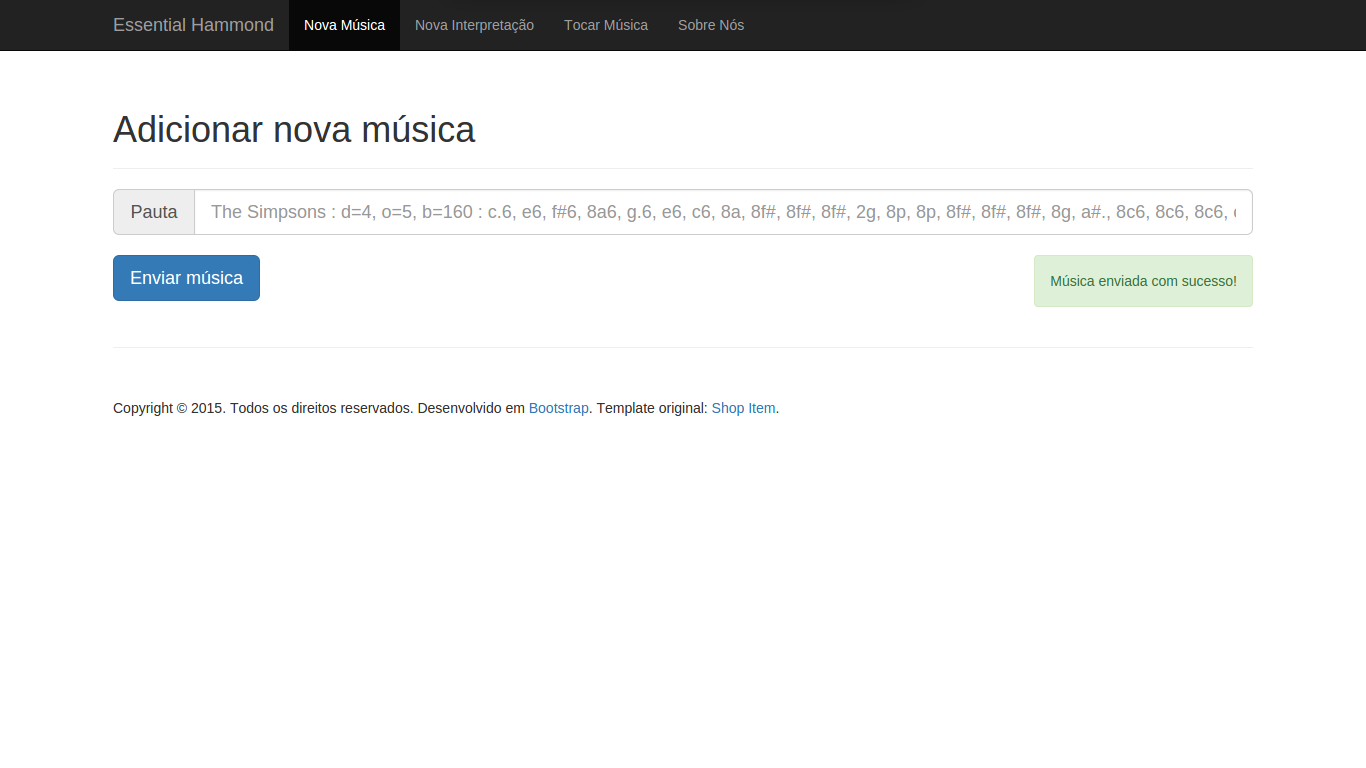
\includegraphics[width=\textwidth]{images/desknova.png}}
\caption{Página para adicionar uma nova música na versão desktop da aplicação.}
\label{desknova}
\end{figure}

\subsection{Nova Interpretação}
Tem um funcionamento semelhante à págna anterior, com a existêcia de mais opções para escolher: nome desejado para a interpretação, música a escolher de entre as existes, efeito e registo. Mostra igalmente mensagens de aviso, sendo que na \autoref{deskinter} é possível ver a mensagem intermédia "A Enviar...". São utilizados os serviços /createInterpretation (para enviar a interpretação para o servidor) e /listNotes (para listar as músicas existentes).

\begin{figure}[htp]
\centering
\frame{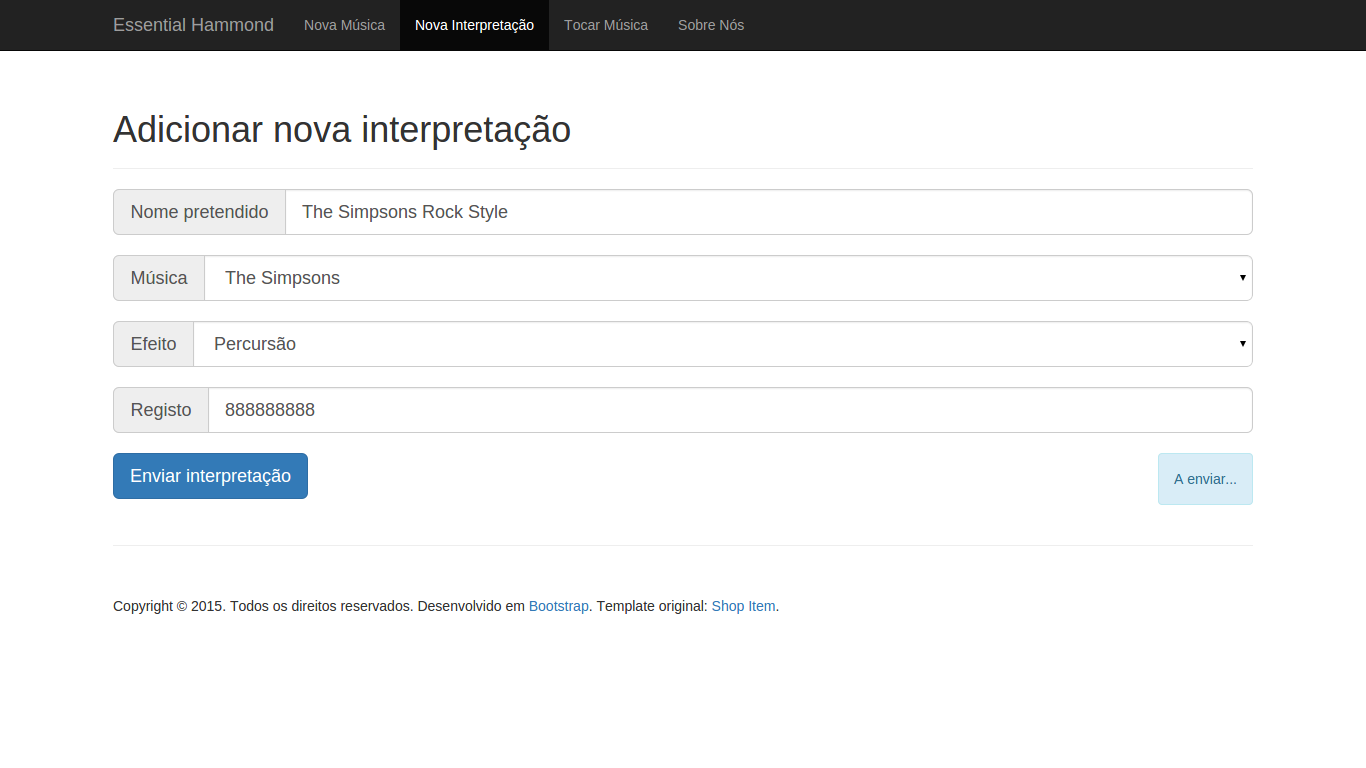
\includegraphics[width=\textwidth]{images/deskinter.png}}
\caption{Página para adicionar uma nova interpretação na versão desktop da aplicação.}
\label{deskinter}
\end{figure}

\subsection{Tocar música}
Esta página dispõe de um menu lateral onde se pode selecionar a música pretendida. Para cada música, é mostrada a imagem da pauta e as respetivas interpretações existentes, com a possibilidade de efetuar votos (ver \autoref{desktocar}). São utilizados os serviços /addVote (para enviar um voto positivo), /delVote (para enviar um voto negativo), /getWaveForm (para obter o ficheiro de som), /getWaveFile (para obter a imagem da pauta), /listNotes (para listas as músicas existentes) e /listSongs (para listar as interpretações exitentes).

\begin{figure}[htp]
\centering
\frame{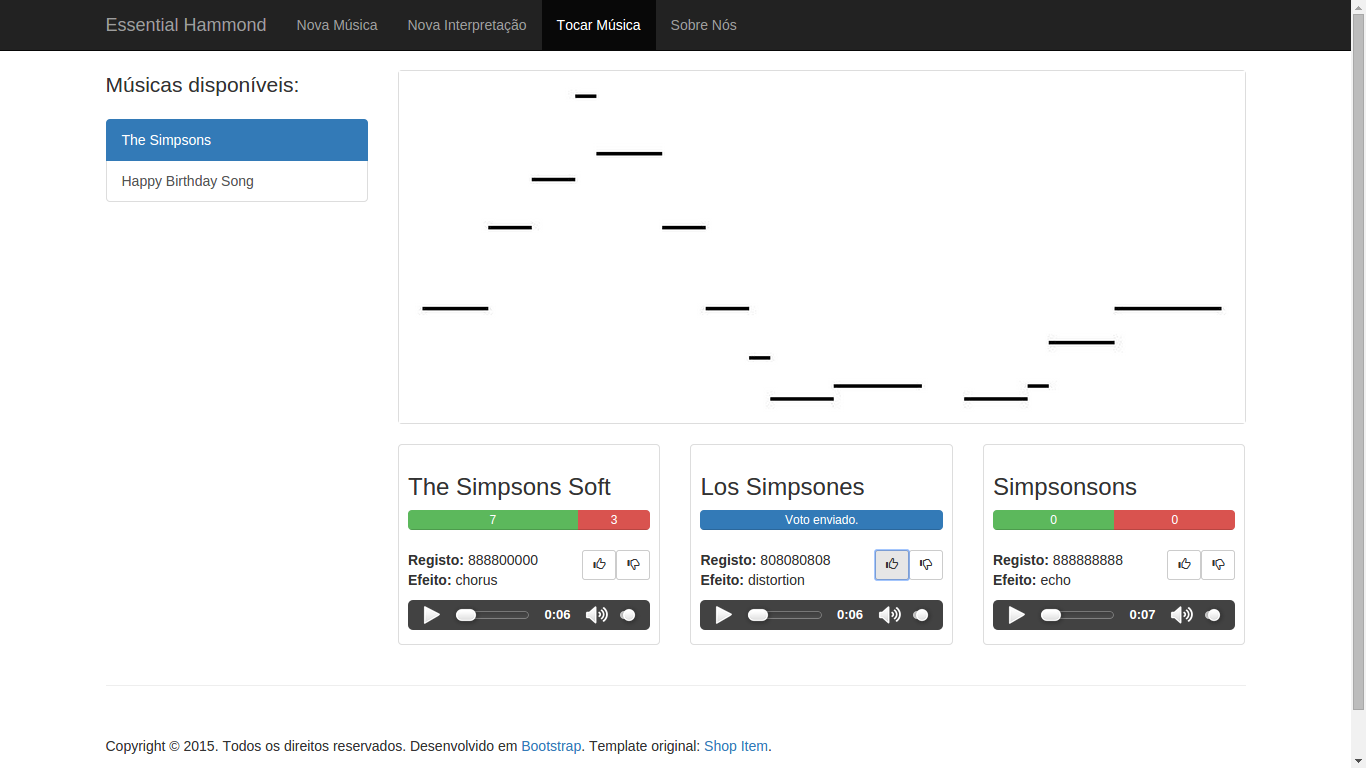
\includegraphics[width=\textwidth]{images/desktocar.png}}
\caption{Página para reproduzir músicas na versão desktop da aplicação.}
\label{desktocar}
\end{figure}

\subsection{Sobre nós}
Disponibiliza informação sobre os quatro elementos do grupo, apresentando também os agradecimentos a quem colaborou com sugestões no nosso projeto (ver \autoref{desksobre}).

\begin{figure}[htp]
\centering
\frame{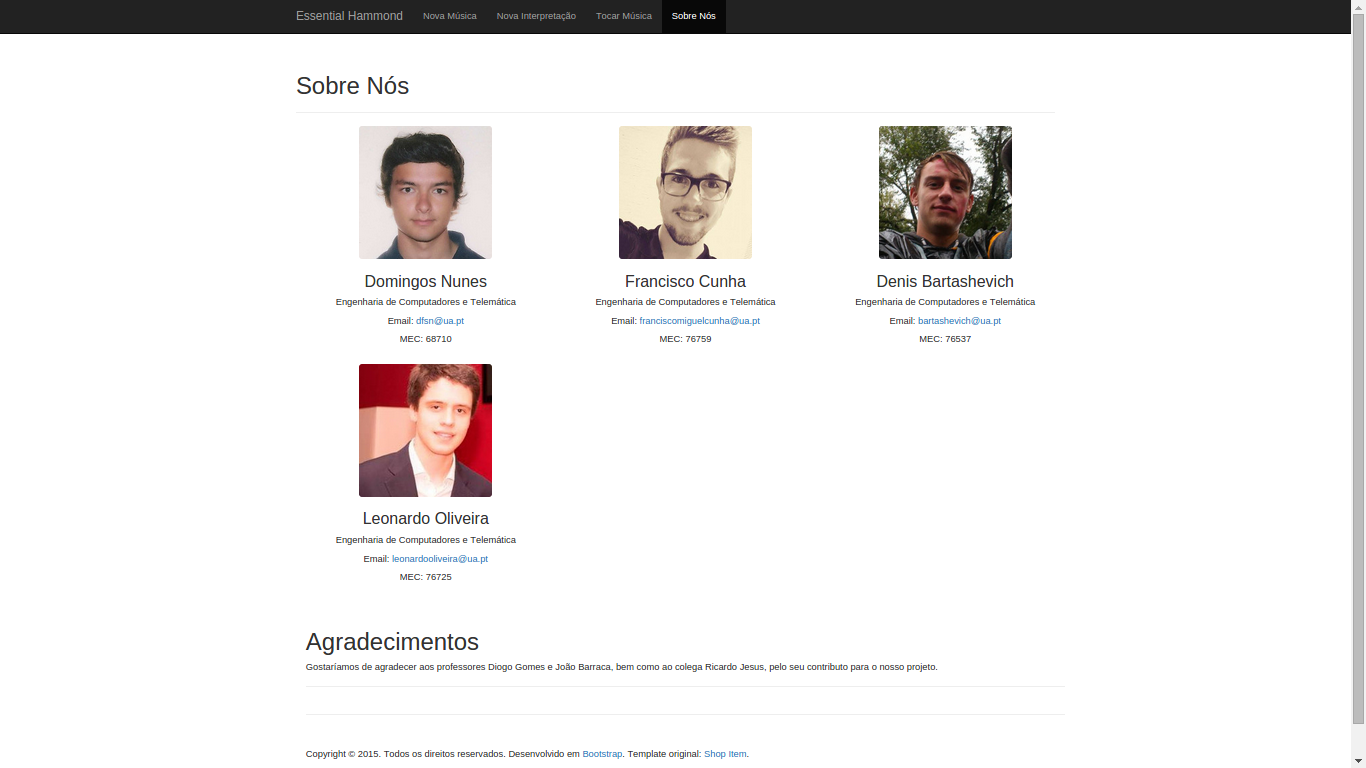
\includegraphics[width=\textwidth]{images/desksobre.png}}
\caption{Página com informação dos elementos do grupo e agradecimentos.}
\label{desksobre}
\end{figure}